%\documentclass{article}
%\documentclass[aps,prl,amssymb,amsmath,twocolumn,floatfix]{revtex4}
\documentclass{jpconf}
\usepackage{graphicx}
\usepackage{amsmath}
\usepackage{amssymb}
\usepackage{lmodern}


\begin{document}
\title{Interfaces in the evolutionary games}
\author{Sergei Kolotev$^{1, 2}$, Aleksandr Malyutin$^{1}$, Evgeni Burovski$^{1, 2}$, Lev Shchur$^{1, 2, 3}$}
\address{$^1$ National Research University Higher School of Economics, 101000 Moscow, Russia}
\address{$^2$ Science Center in Chernogolovka, 142432 Chernogolovka, Russia} 
\address{$^3$ Landau Institute for Theoretical Physics, 142432 Chernogolovka, Russia}

\begin{abstract}
We investigate geometrical aspects in a spatial evolutionary game. The game is based on the prisoner's dilemma. 
Geometrical structure of the space distribution of cooperators and defectors in the steady-state regime of evolution is analyzed. 
We develop algorithm for the identification of the interfaces between clusters of cooperators and defectors, and measure fractal properties of the interfaces.
\end{abstract}



\section{Introduction} 

Last years much interest was payed to the investigation of the physical and mathematical properties of interfaces in the plane
and to the identification of the origin of the phase transitions. The interest is due to the two main factors, the scientific factor and the practical factor. 
First, it is development of the SLE (Stochastic Loewner Evolution~\cite{Shramm2000}, named later as Shcramm-Loewner Evolution) which connects 
properties of the random walk in the upper half-plane with the properties of Conformal Field Theory (CFT)~\cite{BPZ}. 
It turns out to be the third alternative (in addition to the algebraic solution~\cite{Baxter}  and to CFT solution~\cite{DF}) to solve critical properties of some two-dimensional systems of classical statistical physics. Among successful examples are  percolation problem~\cite{Shramm2001,Smirnov2001} and Ising model~\cite{Smirnov2010}. Second, interest to the investigation of the physics and mathematics in two-dimensional geometry is connected to the practical problem of the development of new materials for the next generation of microelectronic devices~\cite{Example-for-2D}. 

In the paper, we focus on the analysis of geometrical properties of interfaces, emerging in the steady-state regime of the space-evolutionary game~\cite{Nowak1992,Nowak2006}. It is the game played by $L^2$ agents arranged on an $L{\times}L$ rectangular lattice with periodic boundary conditions. At each instant of time, each player can be in a state of a cooperator $C$ or a defector $D$. Each agent compute his strategy to keep his current state, or change it depending on the payoff computed as the sum of his pair interaction with the neighbors. This is done for all agents in parallel. The new state is assigned for all neighbors and time is incremented by one. It was found in~\cite{Nowak1993} that starting with some initial distribution, system goes to some steady-state distribution of cooperators and defectors. They found also that starting from some regular distribution of agents the regular self-similar structures appeared, while the random initial conditions leads to some random steady-state structures, and final steady-state stage depend on the payoff parameter. 

It is natural to ask, what is the geometrical structure of the steady-state random fractal? In particular, what is the fractal dimension of the interfaces between clusters of cooperators and defectors? The answer can be informative for the possible classification of the changes of the steady-state stages while tuning payoff parameter.

In the theory of the phase transitions~\cite{Stanley}, there are two most investigated cases, the second-order phase transition, and first-order phase transition. In the two dimensional configurational space, in the case of second-order transition, the interface length $\cal L$ scales with the systems size $L$ as power law ${\cal L}\propto L^{\theta}$~\cite{Barber}. In the case of the first-order phase transition, the interface of droplets scales linearly ${\cal L}\propto L$~\cite{Binder}. Last years, the mixed phase transitions are discussed with the only analytically investigated example on transition in the one-dimensional space~\cite{Bar-Mukamel}, in which some observables behaves like in the first-order phase transitions, and another one as in the second-order phase transitions. In usual percolation, probability to belong to the infinite cluster behaves as power law of the parameter of the model. It was argued by some authors that in dynamical percolation, these probability can change sharply while change parameter~\cite{Adler}, and this is known now as discontinuous percolation~\cite{Herrmann}. We do not aware on the any analysis of the interfaces in these nontrivial cases.

The steady-state structures does percolate for some range of values of the payoff parameter, thus demonstrating some correlated behavior of agents like in the case of second-order phase transition. There are sharp changes of the observables while changing value of the payoff parameter like in the case of first-order phase transition. At the same time, our model is not statistical mechanical model with thermodynamic equilibrium and fluctuations. The steady-state regime achieved not as equilibration process and rather as dynamical process. So, the steady-state structures is the self-organized ones. 

Paper is organized as follows. In Section~\ref{sec:model} we describe model and review some previously known results which is important for the discussion. In Section~\ref{sec:algorithms} we describe algorithms we apply for the simulations and analysis. In Section~\ref{sec:results} we present results of simulations and analysis of the data. In section~\ref{sec:conclusion} we discuss results and future work.

\begin{figure}
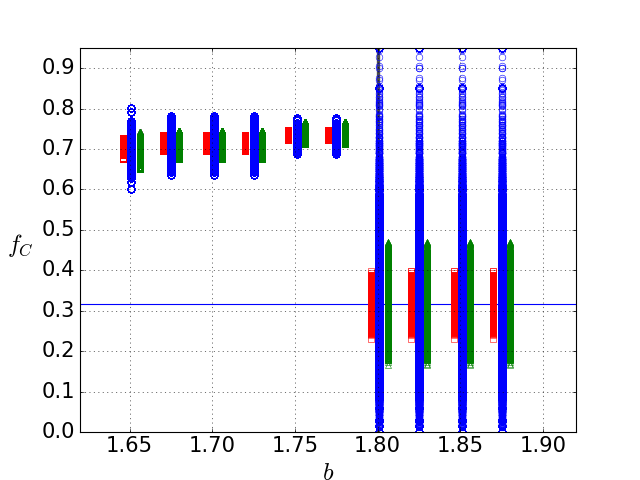
\includegraphics[width=0.5\columnwidth, keepaspectratio=True]{fig1_1.png}~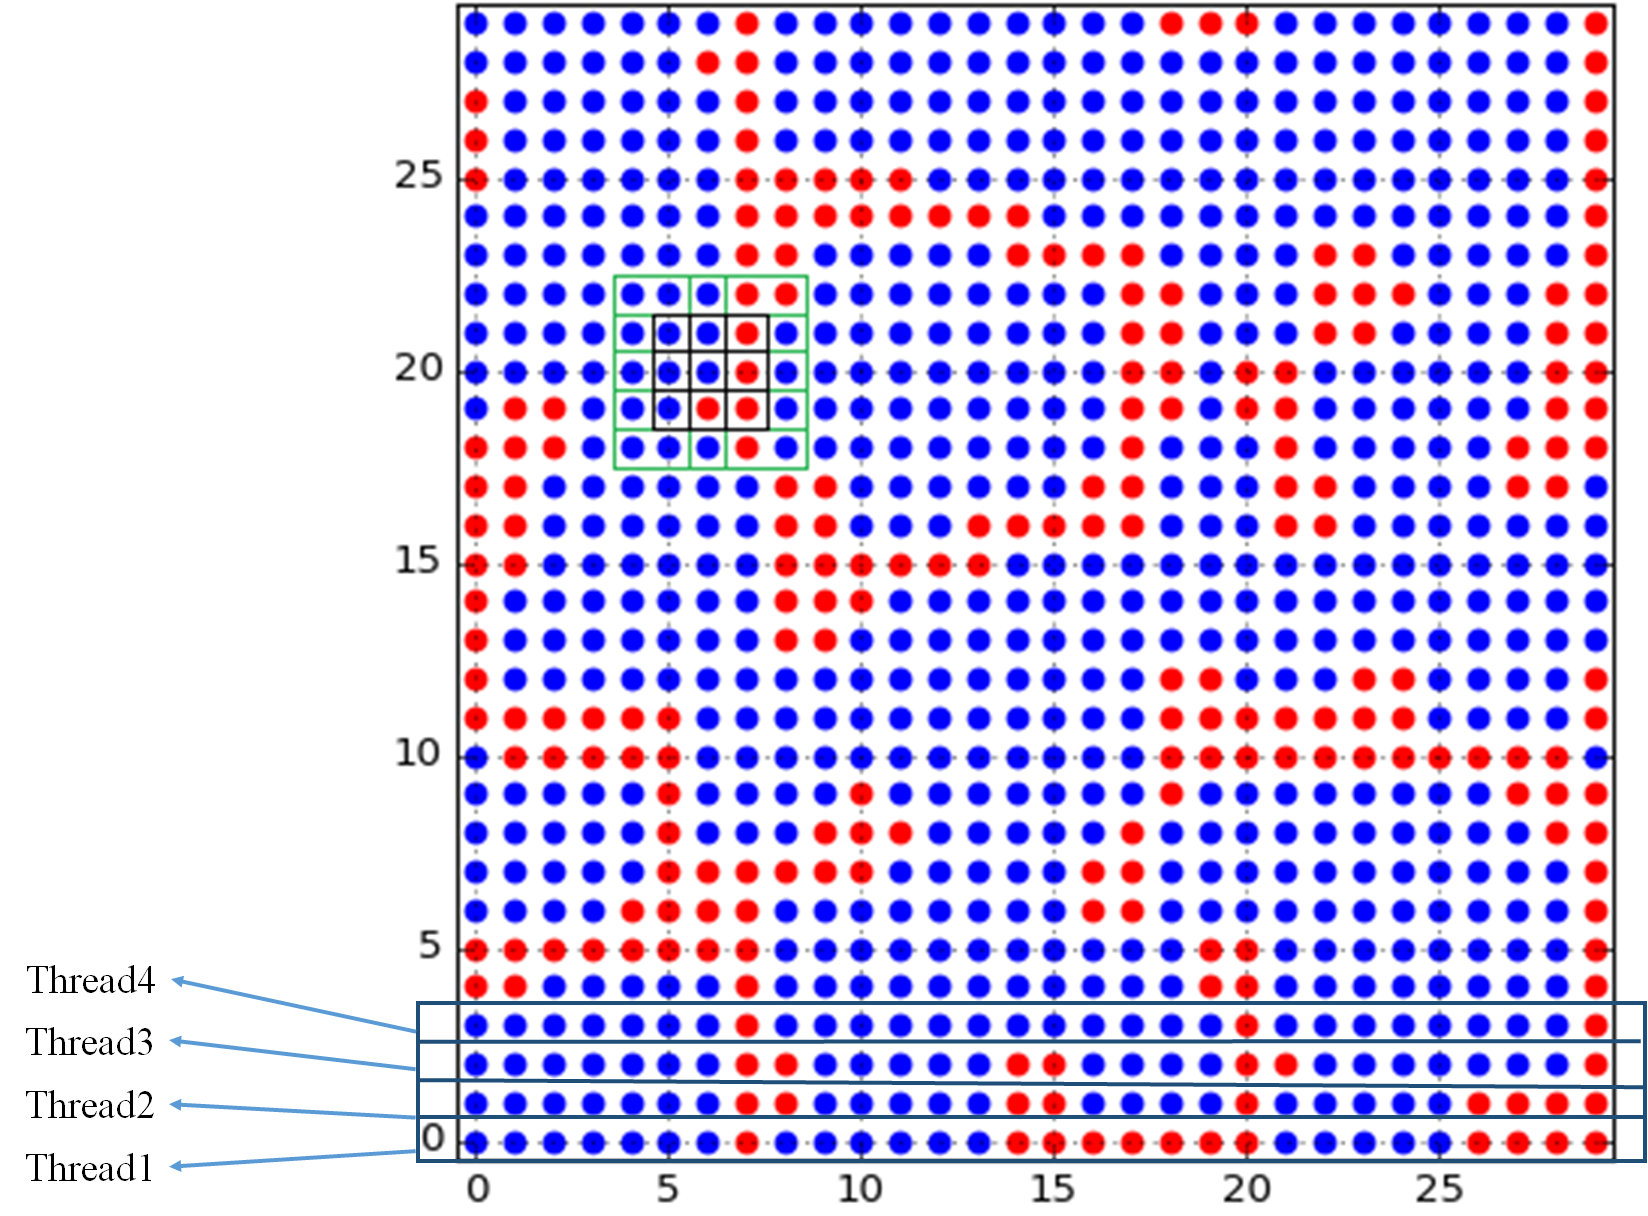
\includegraphics[width=0.5\columnwidth, keepaspectratio=True]{rule.png}
\caption{{\bf Left}: Concentration of cooperators $\mathcal C$, $f_C$, as function of the payoff parameter $b$ for the lattice 
sizes 20x20 (blue), 50x50 (green), and 100x100 (red). 
For clarity, green signs are shifted horizontally slightly to the right and
red signs are shifted to the left. All simulations are performed at
$b =1.651, 1.675, 1.701, 1.725, 1.751, 1.775, 1.801, 1.825, 1.851, 1.875$. 
%
Each point is a single measurement in a simulation of 2$\times 10^4$ generations
of 25 independent realizations of initial conditions.
%
Blue line denotes the magic value $f_C = 12\,\log{2} - 8 \approx 0.318$ \cite{Nowak1993}.
See text for discussion. {\bf Change label T to b. Check values of b at which points are calculated.}\\
{\bf Right}: Illustration of the association of the lattice vertices and threads. Also shown the vertices with coordinates 
(6,20) surrounded by the neighbors influenced on his decision on the next time step.}
\label{fig:density}
\end{figure}


\section{Model of space evolution game}
\label{sec:model}

A prototypical model of the game theory is the so-called \emph{Prisoner's dilemma} (PD),
played by two agents in discrete time steps. In each round of the game, each
player uses one of two possible strategies, \emph{cooperate}, $\mathcal{C}$, or
\emph{defect}, $\mathcal{D}$, and receives a payoff which depends
on the strategies of the player and its opponent~\cite{Tadelis2013}.  We use the following payoff structure
\cite{Nowak1992, Nowak1993}: (i) If two players are $\mathcal{D}$ , they receive nothing; 
(ii) If both players $\mathcal{C}$, each of them receives a payoff of $S$, which
we set to $S=1$ without loss of generality; (iii) In the interaction of
$\mathcal{C}$ and $\mathcal{D}$, the $\mathcal{D}$ receives a payoff $T > S$ and the
$\mathcal{C}$ receives zero. This way, the payoff structure only depends on a
single parameter, the payoff parameter $b = T/S$. We put $S=1$ without loss of generality. 

The game starts with some initial configuration of $\mathcal{C}$ and $\mathcal{D}$ placed in the vertices of the square rectangular lattice with periodic boundary conditions, i.e. it is square lattice on the tori with $L{\times}L$ vertices. Each agent compute payoff of his ``interaction'' with 8 neighbours (in a way chess king's moves) and with itself using the above rule for pair interaction. Payoff is calculated as some of the pair-wise payoff parameters. In the next time step (next generation, on the language of the game~\cite{Nowak1993}), an agent changes her strategy to those one neighbours (including itself) that received the highest payoff. Thus the cell future depend on the mind of the cell, the 8 neighbours and their neighbours, altogether these are 25.  




The dynamical behaviour depends on the value of the payoff parameter $b$. Possible payoffs of agents can take only discrete values of the form $i+bj$, therefore the different regimes can be occurred at some discrete set of $b$ values~\cite{Nowak1993}. We concentrate our analysis for the narrow range of $3/2<b<2$, which we find the most interesting. In this range, in the steady-state regime, concentration of $\mathcal C$ is changed, as can be seen in the Figure~\cite{fig:density}. It is clearly visible that average concentration of $\mathcal C$ in the steady-state regime changes at the values of $b=3/2,8/5,5/3,7/4$ and $9/5$. This values is explained~\cite{}  which corresponds to the different oscillators of small size and with the short period of oscillations. 

Data for the Figure~\ref{fig:density} was obtained starting with sufficiently dense and random initial configuration of $\mathcal C$ and $\mathcal D$, f.e. $f_c=0.9$ and $F_D=0.1$. Spread of the data can be clearly attributed to the finite size of the system, as red signs are spread less than green signs, and green signs is less than the blue signs. Spatial distribution of the steady-state structures are shown in the Figure~\ref{fig:snapshots} as snapshots at some random time step. It can be seen that in the left figure there are blue path (corresponding to $\mathcal C$) from one side to another side of the lattice. Another words, blue cluster percolates, and in the ``thermodynamic limit'' ($L\rightarrow\infty$) will be infinite. At the right figure, the red cluster percolates. Clearly, something happens at the critical value $b=9/5$. It is known~\cite{Nowak1993} that for $b>9/5$ square with nine  $\mathcal D$ can grow in the sea of the $\mathcal C$. Due to the random initial condition, system is self organized to the one of the steady state like in the right Figure~\ref{fig:snapshots}, and average concentration is just the magic value $f_C = 12\,\log{2} - 8 \approx 0.318$ calculated for the 9 $\mathcal D$ in the reference~\cite{Nowak1993}.

\begin{figure}
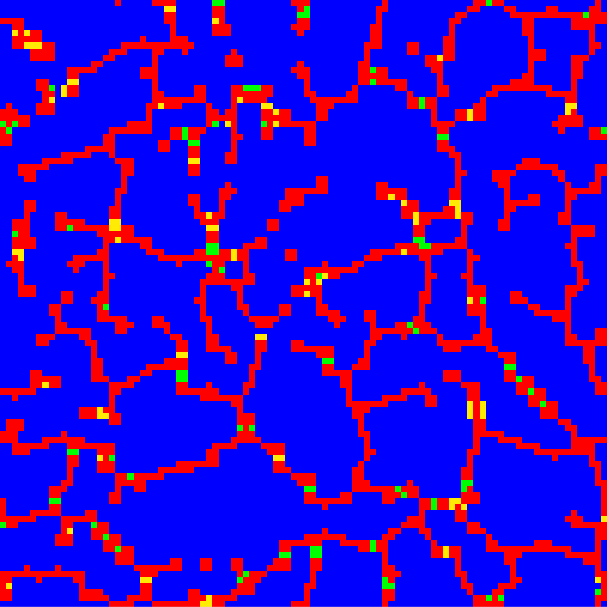
\includegraphics[width=0.5\columnwidth, keepaspectratio=True]{179.png}~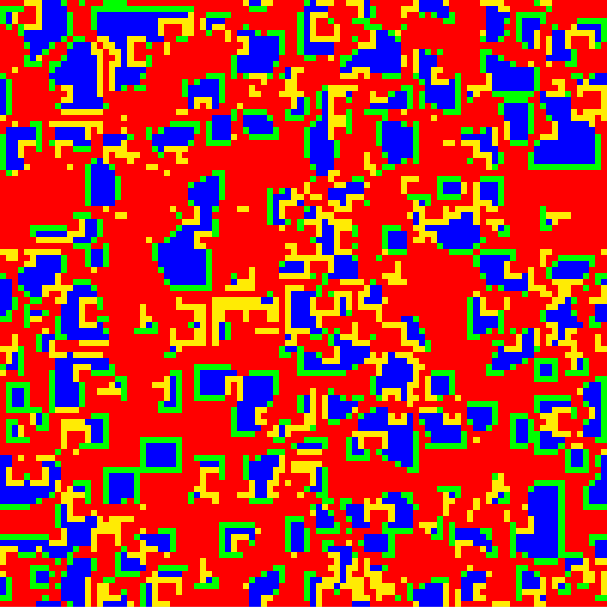
\includegraphics[width=0.5\columnwidth, keepaspectratio=True]{181.png}
%
\caption{Snapshots of the game field for $b=1.79$ (left)
and $b=1.81$ (right). The color coding is consistent with Ref.\ \cite{Nowak1992, Nowak1993}:
blue is $\mathcal{C}$, red is $\mathcal{D}$, yellow is a $\mathcal{D}$ which was
a $\mathcal{C}$ in the previous round, and green is a $\mathcal{C}$ which was
a $\mathcal{D}$ in the previous round. See text for discussion.
}
\label{fig:snapshots}
\end{figure}




\section{Algorithms}
\label{sec:algorithms}

We use OpenMP to accelerate simulations. Each row of the lattice processed by a thread as shown in the right Figure~\ref{fig:density}. {\bf to Serge Kolotev - what is acceleration? Do you have some table, etc.?}

We use Hoshen-Kopelman algorithm, which provide exact decomposition of the game on the clusters of $\mathcal C$ neigbors and  $\mathcal D$ neigbors. Left figure~\ref{fig:alg} illustrates how it works. We start with the upper-left site (0,0) and assign it to the $\mathcal C$ cluster number 1. Then we check the next site in the row (0,1), which is connected (as a neigbor to the cite (0,0)) and assign it to the same cluster number 1. The same happens with the third site (0,2). The forth site (0,3) is $\mathcal D$ site, and we assign it to the cluster number 2, and so on. Figure shows what happens if algorithm scanning lattice row-by-row arrives to check site (6,4). Left neigbor belongs to the cluster 1, and upper site belongs to the cluster 3. Site (6,4) will be assigned to the cluster 1, as well as all sites assigned to the moment to the cluster 3, will be reassigned to the cluster 1. Process of reassignment is generated by the red arrow. After decomposition is finished, we calculate cluster masses (or sizes) as number of sites in each cluster, and updated histogram of the cluster sizes.

We use procedure of ref.~\cite{ZS2010} to extract interface between $\mathcal C$-clusters and $\mathcal D$-clusters. It is defined on the dual lattice, which is plotted through the middle of the edges connecting sites, and perpendicular to them. It is illustrated in the right Figure~\ref{fig:alg}. We extract external interface of the percolating cluster (it is $\mathcal C$-cluster in the figure), and calculate average length $\mathcal L$ , which is the average length of the percolating interfaces in the steady-state regime. If lattice do not contain percolating interface, we do not update averages. 

\begin{figure}
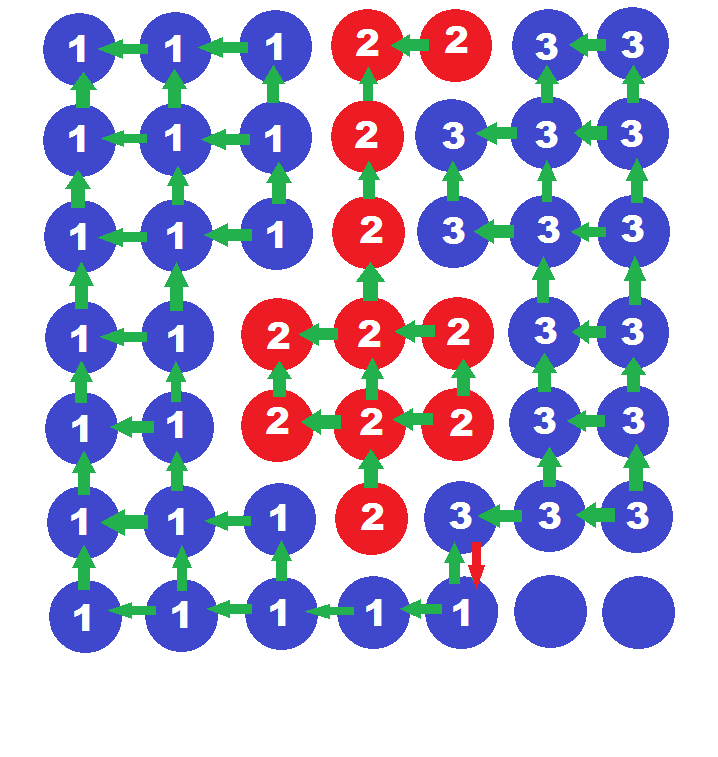
\includegraphics[width=0.5\columnwidth, keepaspectratio=True]{HKpic2.png}~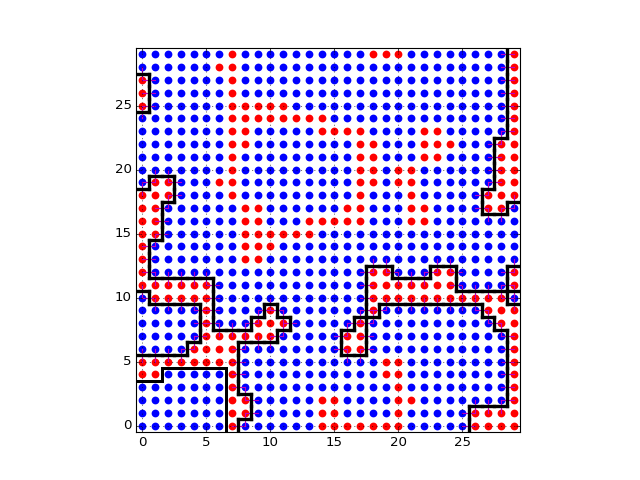
\includegraphics[width=0.5\columnwidth, keepaspectratio=True]{border2.png}
%
\caption{Left: illustration of Hoshen-Kopelman algorithm. Right: illustration of interface extraction.
}
\label{fig:alg}
\end{figure}

\section{Results of simulations and data analysis}
\label{sec:results}

The average density of $\mathcal C$ changed drastically from the value $f_c=0.737(6)$ at $b=1.775$ to the value $f_c=0.315(6)$ at $b=1.825$ (see Figure~\ref{fig:density}). We have to stress that magic density which corresponds to the growth of $\mathcal D$ cluster is $f_c=12\log 2-8\approx 0.318$. So, we can attribute transition from the $\mathcal C$-cluster (blue one in the left Figure~\ref{fig:snapshots}) percolation at $3/2<b<9/5$ to the transition of the  $\mathcal D$ (red one in the right Figure~\ref{fig:snapshots}) to the transition from the random oscillatory regime of $\mathcal C$-clusters to the random growth regime of $\mathcal D$-clusters. Denisty changes abruptly at $b=b_c=9/5$.

Cluster size distribution in both cases demonstrate exponential decay of the sizes with the lattice growth, although range of the distribution is much large in the case of 
$\mathcal D$-clusters proliferation. 

We fit interface length $\mathcal L$ to the power law

\begin{equation}
{\mathcal L} = A L^\theta +c.
\label{eq:power}
\end{equation}
The result for $b=1.74$ is $A=0.22(4)$, $c=5(9)$, and $\theta=2.07(5)$. For $b=1.81$ it is $A=0.35(1)$, $c=-20(5)$, and $\theta=1.99(1)$. Values of $c$ is not important although it give some idea of the typical correlation length, but accuracy is not enough for any definite conclusions. What is very intriguing is that the interface of the percolating clusters in both regimes is close to 2, which is not obvious while looking in the Figures~\ref{fig:snapshots}. Value of $\theta=2$ corresponds to the line which is space-filling in the thermodynamic limit of $L\rightarrow\infty$.

To check this finding we estimate Minkowski dimension, covering interface with the boxes of size $l$, counting number of boxes $N(l)$,  and get limit of $l\rightarrow 0$
\begin{equation}
d_M=\lim_{l\rightarrow 0} \frac{log\; N(l)}{-log\; l}.
\label{eq:boxes}
\end{equation}
This quantity is much more sensitive to the finite size of the lattice $L$ as well there are visible deviations for the box sizes $l$ comparable with the lattice spacing, which is 1. We fit data for $N(l)$ with the linear formula
\begin{equation}
\log\; N(l)=B\log\; (1/l)+c.
\label{eq:power}
\end{equation}
Results is presented in the Table~\ref{tab}. There are clear tendency of $d_M$ to the value of 2. 

\begin{table}
\center
\begin{tabular}{rrrr}
$L$  & $d_M (b = 1.79)$ & $d_M (b=1.81)$ \\
\hline
100 & 1.78 & 1.38 \\
200 & 1.76 & 1.76 \\
500 & 1.94 & 1.94 \\
1000 & 1.96 & 1.96 \\
\end{tabular}
\caption{Estimation of the Minkowski dimension $d_M$ of the interface.}  
\label{tab}
\end{table} 


\section{Discussion and future work}
\label{sec:conclusion}


We study an evolutionary game bases on a Prisoner's Dilemma with short-memory players arranged on a square grid in two spatial dimensions. Despite its apparent simplicity, this deterministic, globally synchronous game displays surpirzingly rich behavior in the long time limit: The steady state of the game features a series of dynamic regimes separated by the sharp transitions at specific values of the payoff parameter. The transitions are characterized by jumps of the average density of cooperators, and non-trivial rearrangements of the game field. The interfaces between clusters of strategies are stochastic fractals, which, however, are space-filling across the transitions, thus resembling specific Julia sets which are also space-filling \cite{Shishikura1998}.

It would be interesting to further characterize these emergent geometric structures.
It would also be interesting to investigate the game for more complicated arrangements of players, such as non-square grids, complex networks and dynamic graphs.



\ack
We thank Lev Barash for helpfull discussions. This work was supported by
RFBR grant 16-07-01122  (section~\ref{sec:algorithms})  and grant 14-21-00158 from the Russian Science Foundation.

%%%%%%%%%%%%%%%%%%%%%%%%%%%%%%%%%%%%%%%%%%%%%%%%%%%%%%%%%%%%%%%%%%%%%%%%%%%%%
\section*{Refrences}
\begin{thebibliography}{99}

\bibitem{Shramm2000} O. Schramm, \textit{Scaling limits of loop-erased random walks and uniform spanning trees}, Isr. J. Math. {\bf 118}, 221 (2000).

\bibitem{Shramm2001} O. Schramm and S. Sheffield,  \textit{Harmonic Explorer and Its Convergence to $SLE_4$}, The Annals of Probability {\bf 33}, 2127 (2005).

\bibitem{Smirnov2001} S. Smirnov, {\textit Critical percolation in the plane: conformal invariance, Cardy's formula, scaling limits}, Comptes Rendus de l'Acad�mie des Sciences {\bf 333}, 239 (2001).

\bibitem{Smirnov2010} S. Smirnov, {\textit Conformal invariance in random cluster models. I. Holomorphic fermions in the Ising model}, Ann. Math., {\bf 172}, 1435 (2010). 

\bibitem{Example-for-2D} Example of 2D structures - some review

\bibitem{BPZ}  A. A. Belavin, A. M. Polyakov, and A. B. Zamolodchikov, \textit{Infinite conformal symmetry in two-dimensional quantum field theory}, Nucl. Phys. B {\bf 241} 333  (1984).

\bibitem{Baxter} R.J. Baxter, \textit{Exactly solvable models in statistical mechanics}, Academic Press, London, 1982. 

\bibitem{DF} Vl.S. Dotsenko, V.A. Fateev, \textit{Conformal algebra and multipoint correlation functions in 2D statistical models}, Nucl. Phys. B {\bf 240 (FS12)}, 312 (1984).

\bibitem{Nowak1992} M.A. Nowak and R.M. May, \textit{Evolutionary games and spatial chaos}, Nature {\bf 359}, 826 (1992).

\bibitem{Nowak2006} M.A. Nowak,  \textit{Evolutionary Dynamics: Exploring the equations of life}, The Belknap Press, (2006).

\bibitem{Nowak1993} M.A. Nowak and R.M. May,  \textit{The spatial dilemmas of evolution}, Int. J. Birurcation and Chaos {\bf 3}, 35 (1993).

\bibitem{Stanley} H.E. Stanley, \textit{Introduction to phase transition and critical phenomena}, Oxford University Press {1971}.

\bibitem{Barber} M.N. Barber, \textit{Finite size scaling}, in Phase transitions and critical phenomena, Eds. C. Domb and J Lebowitz, volume 8 (1983).

\bibitem{Binder} K. Binder, \textit{Theory of first-order phase transitions}, Rep. Prog. Phys. {\bf 50}, 783 (1987).

\bibitem{Bar-Mukamel} A.~Bar and D.~Mukamel, \textit{Mixed-Order Phase Transition in a One-Dimensional Model}, Phys. Rev. Lett. {\bf 112}, 015701 (2014).

\bibitem{Adler} J. Adler, \textit{Bootstrap percolation}, Physica A {\bf 171}, 453 (1991).

\bibitem{Herrmann} H. Herrmann, \textit{Discontinuous percolation}, J. of Phys: Conf. Series {\bf 681},012003 (2015).

\bibitem{Tadelis2013} see, \textit{e.g.}, S. Tadelis, \textit{Game Theory: An Introduction}, Princeton University Press, 2013, and references therein.








\bibitem{Axelrod81} R.~Axelrod, W.D.~Hamilton, \textit{The Evolution of Cooperation},
Science, \textbf{211}(4489), 1390 (1981).

\bibitem{Axelrod06} see, \textit{e.g.,} R.~Axelrod, \textit{The Evolution of Cooperation}, Basic Books, 2006, and references therein.


\bibitem{Jonker78} P.D.~Taylor and L.B.~Jonker,  \textit{Evolutionary stable
strategies and game dynamics}, Math. Biosci., \textbf{40}(12), 145156 (1978).

\bibitem{Smith82} J. Maynard Smith, \textit{Evolution and the Theory of Games}, 
Cambridge University Press, (1982).

\bibitem{Weibull95} J.W.~Weibull, \textit{Evolutionary Game Theory}, MIT Press, (1995).

\bibitem{Szabo05} C.~Hauert and G.~Szabo, \textit{Game theory and physics},
Am. J. Phys. \textbf{73}(5), 405414 (2005).

\bibitem{Perc09} A.~Szolnoki and M.~Perc, \textit{Emergence of multilevel selection
 in the prisoner's dilemma game on coevolving random networks}, New J. Phys. \textbf{11}, 093033, (2009).

\bibitem{Helbing2013} D.~Helbing, \textit{Globally networked risks and how to
respond}, Nature \textbf{497}, 51 (2013).

\bibitem{Shiff} see, \textit{e.g.,} J.L. Shiff, \textit{Cellular Automata: A Discrete View of the World}, Wiley-Interscience; 1 edition (January 6, 2008), and references therein

\bibitem{ZS2010} A. Zatelepin and L. Shchur, \textit{Duality of critical interfaces in Potts model: numerical check}, arXiv:1008.3573. https://arxiv.org/pdf/1008.3573.pdf


\bibitem{HoshenKopelman} J. Hoshen, R. Kopelman, \textit{Percolation and cluster distribution. I. Cluster multiple labeling technique and critical concentration algorithm}, Phys. Rev. B. \textbf{14}, 8 (1976).

\bibitem{Wang2017} Wenlong Wang, M. A. Moore, Helmut G. Katzgraber, \textit{The
Fractal Dimension of Interfaces in Edwards-Anderson and Long-range Ising Spin
Glasses: Determining the Applicability of Different Theoretical Descriptions},
Phys. Rev. Lett. \textbf{119}, 100602 (2017).

\bibitem{BisoiMishra2001}A.K. Bisoi, J. Mishra, \textit{On calculation of fractal dimension of images}, Pattern Recognition Letters, \textbf{22}, 631 (2001).

\bibitem{JiangLiu2012} S. Jiang, D. Liu, \textit{Box-Counting Dimension of Fractal Urban Form: Stability Issues and Measurement Design}, International Journal of Artificial Life Research, \textbf{3}(3), 41, (2012).

\bibitem{Shishikura1998} M.~Shishikura, \textit{The Hausdorff dimension of the
boundary of the Mandelbrot set and Julia sets}, Annals of Mathematics
\textbf{147}, 225 (1998).


%\bibitem{Review-order} Review with the classification of the phase transitions.

%\bibitem{Review-universality} V.~Privman, P.C.~Hohenberg, and A.~Aharony, \textit{Universal Critical-Point Amplitude Relations}, in \textit{Phase Transitions and Critical Phenomena}, Vol. 14, edited by C. Domb and J.L. Lebowitz (Academic, New York, 1991).

%\bibitem{Binder-review} K.~Binder, \textit{Theory of first-order phase transitions}, Rep. Prog. Phys.,  \textbf{211}, 783 (1987).

%\bibitem{Thouless} D.J.~Thouless, \textit{Long-Range Order in One-Dimensional Ising Systems}, Phys. Rev, \textbf{187}, 732 (1969).

%\bibitem{Bar-Mukamel} A.~Bar and D.~Mukamel, \textit{Mixed-Order Phase Transition in a One-Dimensional Model}, Phys. Rev. Lett., \textbf{112}, 015701 (2014).

%\bibitem{percolation} \textbf{XXX} percolation, some classic reference







\end{thebibliography}


\end{document}


